
\subsection{Answers}
\begin{table}[htb]%
\begin{center}%
\caption{Q8: What is your major role at your place of work?}%
\label{tab:Q8-ans}%
\begin{tabular}{l|l|r}%
\hline%
Choice & Abbrv. & \# Answers \\%
\hline%
{\small Research and development of application(s)} & Apps & 579 (68.4\%) \\%
Performance tuning of MPI program(s) & Tuning & 258 (30.5\%) \\%
Parallelization of sequential program(s) & Parralelize & 237 (28.0\%) \\%
{\small Research and development software tool(s)} & Tools & 222 (26.2\%) \\%
Debugging MPI programs & Debug & 135 (15.9\%) \\%
{\small Research and development on system softw$\cdots$} & OS/R & 126 (14.9\%) \\%
other & - & 61 (7.2\%) \\%
\hline%
\multicolumn{2}{c}{total} & 1618 (847)\\%
\hline%
\end{tabular}%
\end{center}%
\end{table}%


Corroborating the previous question, most of the respondents are developing
applications. Then comes the MPI ecosystem (debugging, tuning, software
tools). A large fraction is working on parallelization and some are working on
research and development of the software stack.
From a country-by-country comparison, the US 
and Japan are more frequently doing research and development 
of OS / Runtime as compared to other countries.

\mycomment[AH]{Thinking the number of answers from Japan, the high ratio
  of OS/R R\&D comes from the biased distribution of the questionnaire.
  There is an active group which is developing XcalableMP, another PGAS
  language. If we could have more number of Japanese answers, then this
  high ratio could be diluted.}

\subsection{List of other answers}
\begin{itemize}
\item Africa: Research and Teaching
\item Asia: Research student
\item Central and South America: HPC Administrator
\item Europe:France: Development of a  multi-thread MPI library
\item Europe:France: Numerical simulation for materials (physics)
\item Europe:France: Research
\item Europe:France: Research in physics
\item Europe:France: Researcher
\item Europe:France: Scientist Researcher in Geophysics
\item Europe:France: associate
\item Europe:France: support
\item Europe:Germany: Academic Research
\item Europe:Germany: Comp. Scientist at HPC site
\item Europe:Germany: Fault-tolerance for future HPC systems
\item Europe:Germany: Management
\item Europe:Germany: Performance analysis
\item Europe:Germany: R\&D of CFD
\item Europe:Germany: Research and development of parallel numerical software
\item Europe:Germany: Research and development of scientific software
\item Europe:Germany: Support and training of researchers
\item Europe:Germany: System administration
\item Europe:Germany: Teaching of MPI and OpenMP
\item Europe:Germany: researcher
\item Europe:Italy: HPC User Support
\item Europe:Italy: RESEARCH IN PHYSICS
\item Europe:Italy: Research scientist
\item Europe:Italy: Teaching at MSc and PhD level, research on parallel and distributed computing
\item Europe:Italy: design and optimization of nonlinear PDE solvers for fluid physics.
\item Europe:UK: HPC Management
\item Europe:UK: Research professor
\item Europe:UK: Science
\item Europe:UK: Scientist
\item Europe:UK: Strategic management and HPC procurement
\item Europe:UK: University Student
\item Europe:others: Advanced user/application support and training
\item Europe:others: Data analysis
\item Europe:others: Management
\item Europe:others: Reaserch (Physics)
\item Europe:others: Resarch
\item Europe:others: Research support
\item Europe:others: Scientific computing
\item Europe:others: Scientist analyst and Code maintainer
\item Europe:others: Scientist: Numerical simulations
\item Europe:others: Support for research
\item Europe:others: Training
\item Europe:others: calculation of a heat storage modell
\item Europe:others: use of programs for image analysis and reconstruction
\item Japan: Manage software at supercomputer center
\item Japan: Research and development on Microarchitecture
\item Japan: Research for genome sequence
\item Japan: System operation and help desk
\item Russia: Application of MPI and non-MPI programs
\item Russia: Scientific HPC solvers for fluid dynamics and quantum physics
\item Russia: System administrator
\item Russia: astrophysical codes
\item Russia: scientist
\item Russia: teaching in physics \& math
\item South Korea: Data Scientist
\item USA: Administration but with some R\&D
\item USA: Developing alternative programming models to MPI
\item USA: Lab head

\end{itemize}

\begin{figure}[htb]
\begin{center}
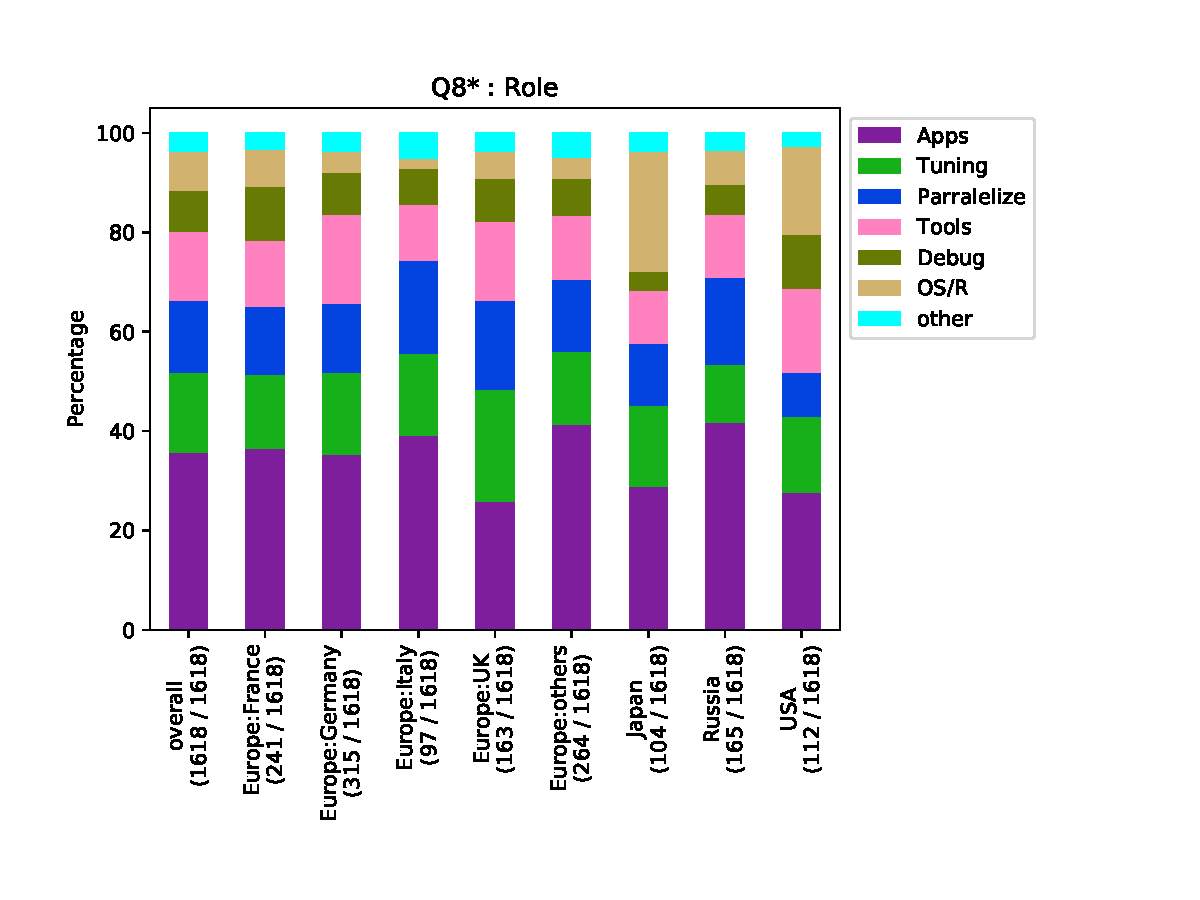
\includegraphics[width=10cm]{../pdfs/Q8.pdf}
\caption{Simple analysis: Q8}
\label{fig:Q8}
\end{center}
\end{figure}
